\subsubsection{MULTI-SCALE 3D INTERPRETATION}
We call multi-scale match to technique here presented 
to track objects that moves in 3 dimensions. 
To understand this technique we need to analyze the same object in 
two different positions, as in the Figure \ref{fig:multiscale3d}.

\begin{figure}[H]
\centering
  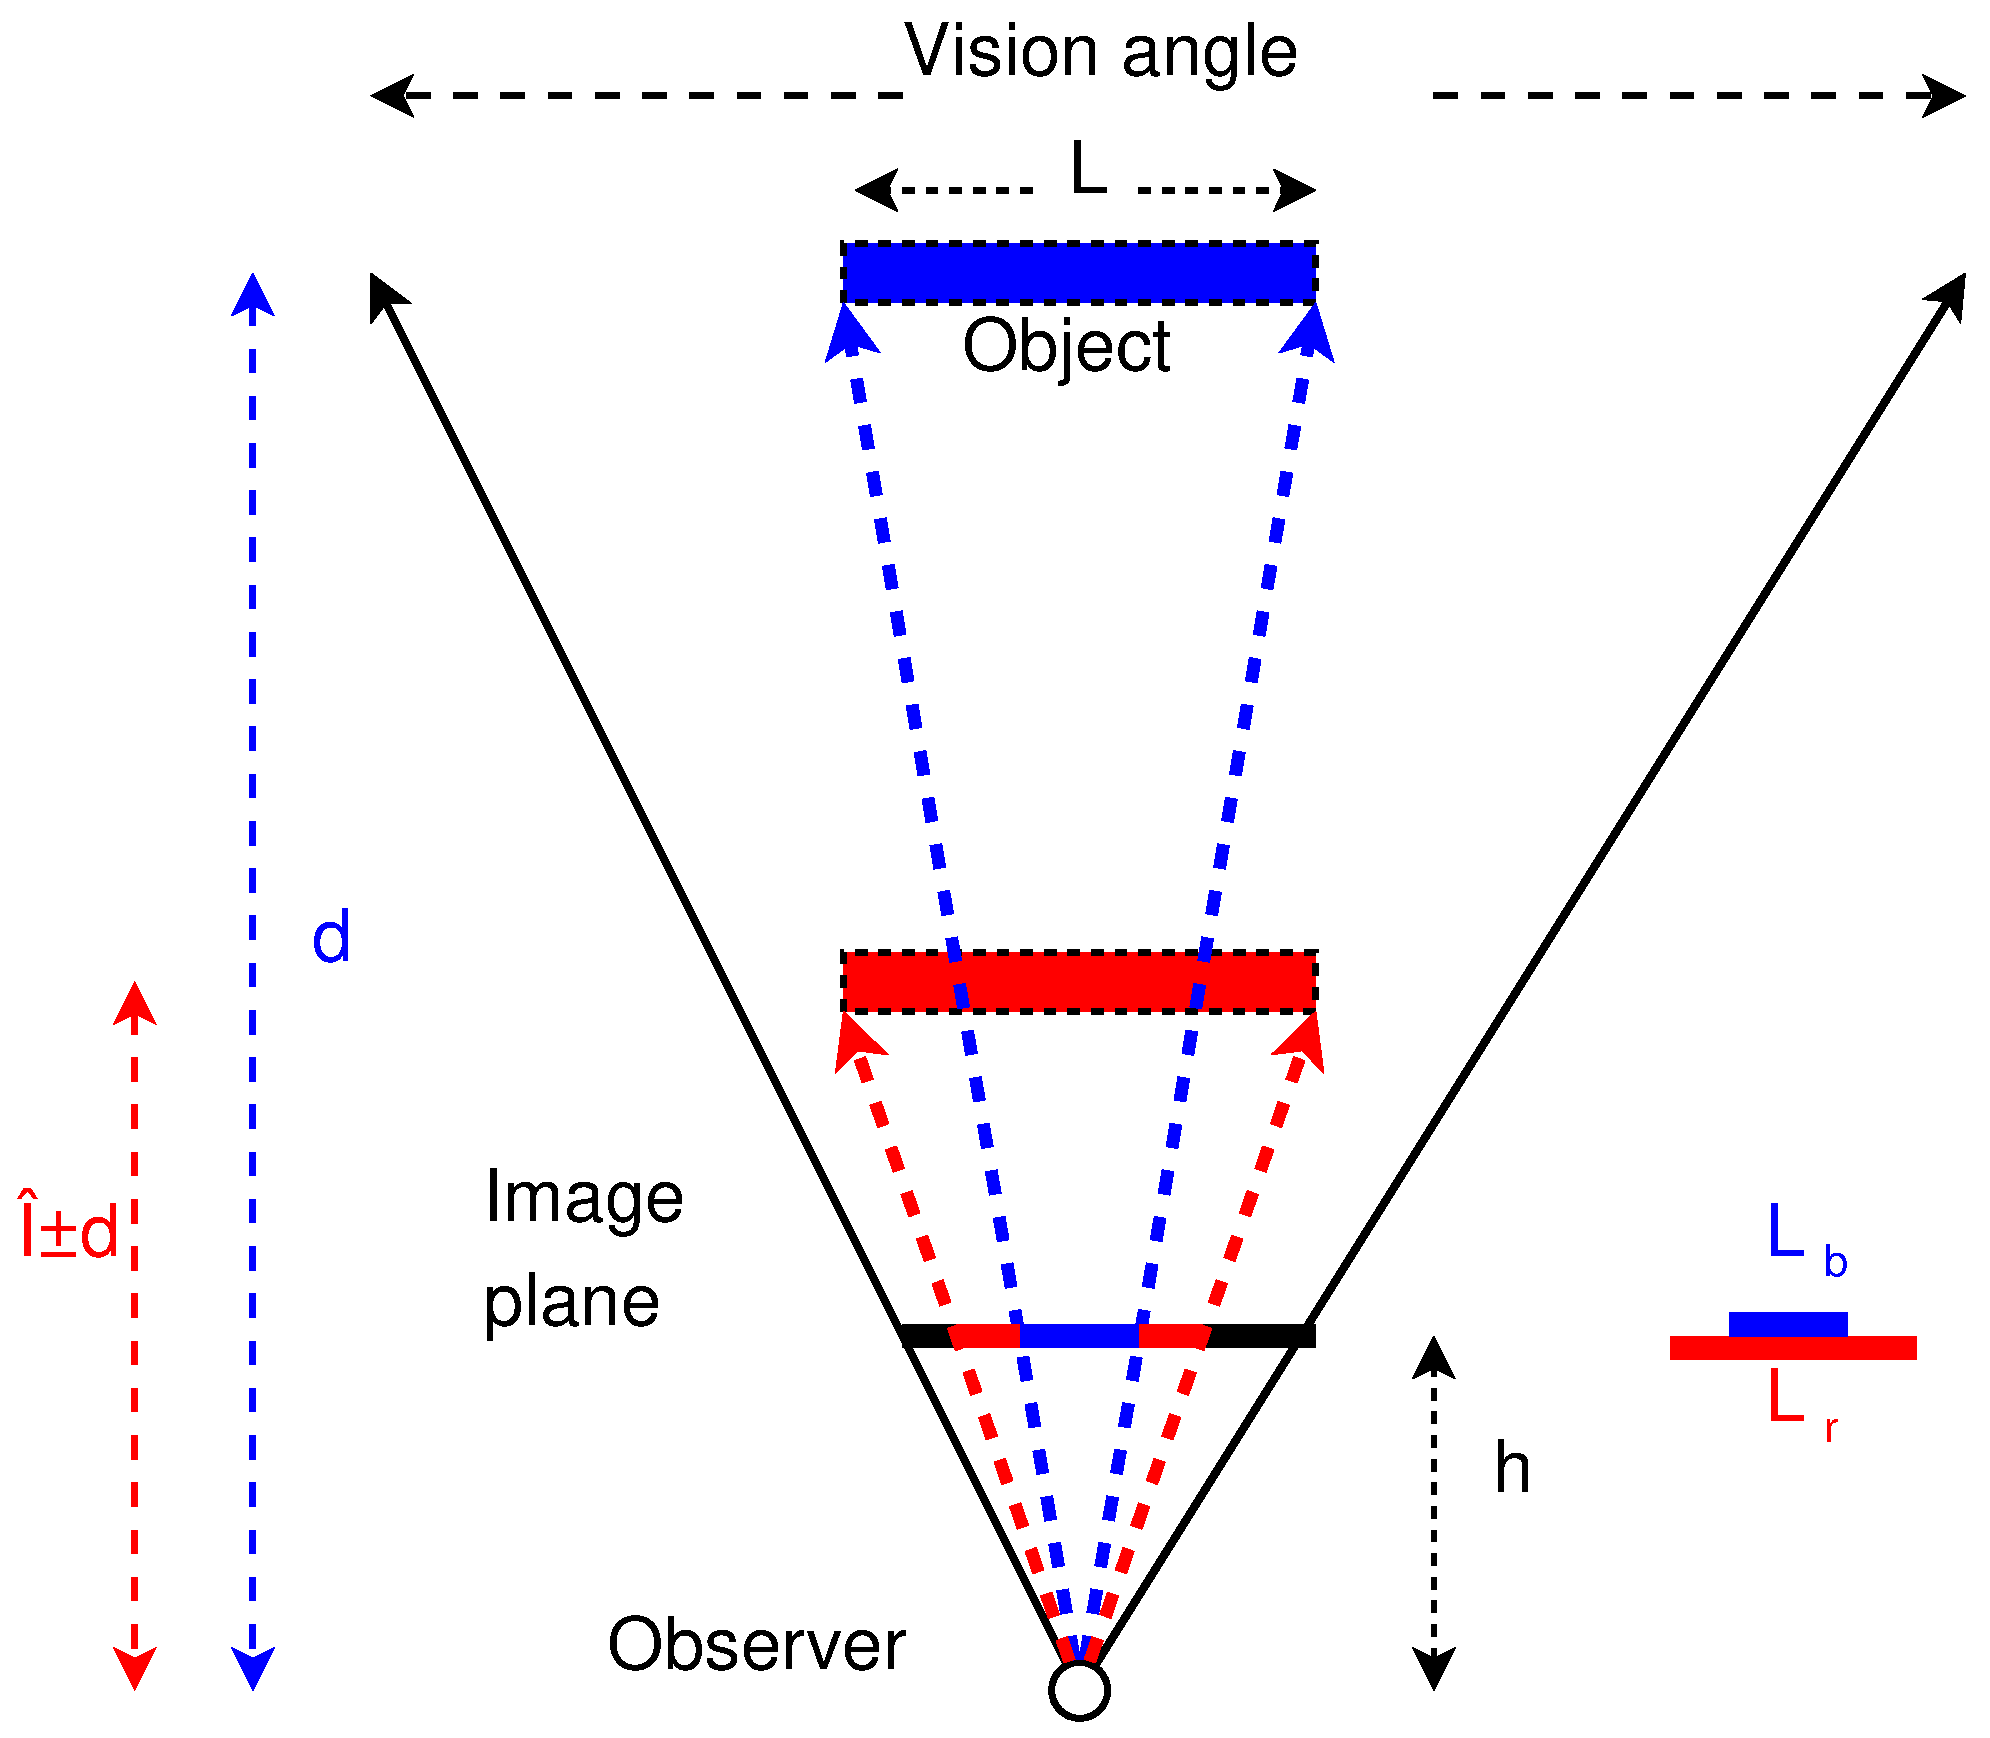
\includegraphics[width=.7\columnwidth]{images/Diagrama3.eps}
  \caption{Interpretation of the area relation in the multi-scale tracking.}
  \label{fig:multiscale3d}
\end{figure}
The figure show, using the colors blue and red, the same object (of width $L$) located at two 
different distances, being these $d$ and $\alpha d$, respectively. 
In both cases, one picture of scene is obtained,
so that, the plane of photography is located at a distance $h$ of observer.
The projections of objects in blue and red, in the plane of photography, are
called of $L_b$ and $L_r$, respectively. Making a simple inspection in the
formed triangles, we can see that $\frac{h}{d}=\frac{L_b}{L}$ and 
$\frac{h}{\alpha d}=\frac{L_r}{L}$, so that $L_b/\alpha= L_r$. 
This imply that \textbf{when an object that is located
at a distance $d$ is relocated to a distance  $\alpha d$, then,
from the point of view of the observer, its width is altered by a factor of $1/\alpha$,
and consequently your area is altered by a factor of $1/\alpha^2$}.

Thus, the multi-scale match criteria, searches the objects
using many discrete values of $\alpha$; so that, each value of $\alpha$
search the object as if this were in a layer nearest or farthest from the observer.
The algorithm try tracking objects nearest with $\alpha<1$ and objects farthest with $\alpha>1$.

%usa Multi-resolution match criteria e explica isso dos tamanhos

\subsubsection{DEPARTURE FACTOR- RELATIVE VELOCITY}
The departure factor is a dimensionless number related to the rate of approaching 
or departure of an object to the observer. The factor
is determined how showed at equation \ref{eq:relarea},

\begin{equation}\label{eq:relarea}
f_a \equiv \alpha^2 \equiv \frac{Area_r}{Area_f} 
\end{equation}

Where $f_a$ and $\alpha$ are defined as the area factor and departure factor, 
respectively; $Area_r$ is the area of ROI and $Area_f$ 
is the area of analyzed region in the current image frame. 

Thus, if we consider that the object analyzed in the $ROI$ was to a distance $d_0$,
them the object in the analyzed region was to a distance of $\alpha d_0$ (or $\sqrt{f_a} d_0$),
so that if the $i-th$ image was analyzed, then $\alpha_i$ and $d_i=\alpha_i d_0$ will be obtained.

The departure factor, $\alpha_i$, has two interpretations, if the rate of departure increase quickly, 
means that the object is departing. Or the apposite, if factor decreases, the 
object is approaching.

Relative velocity is calculate using a simples equation of kinematic in physics:
\begin{equation}
 v_i = \frac{\Delta s}{\Delta t}= \frac{s_i-s_{i-1}}{\Delta t}.
\end{equation}

Where the vector $v_i$ represent the relative velocity in the i-th image frame, 
$s_i=(x_i,y_i,d_i)$ is the position of match in the i-th image frame
and $\Delta t$ is the sampling time between image frames.
Additionally, we call of velocity of departure factor, $v^d_i$, 
to the scalar number that represent the depth component
of vector $v_i$.

The calculated  $v^d_i$  is relative, for the simple reason that the distance (depth) between the 
camera (observer) and the object in the instant i-th ever will be referenced to $d_0$, the distance of
initial $ROI$ that is established by definition to 1.
Finally, in all cases the position $s_i$ is relative to a moving reference system.

